% thesis using usydthesis.cls - Andrew Mathas 5/2002
\documentclass[BSc]{usydthesis}
% \includeonly{chapt1}
%%%%%%%%%%%%%%%%%%%%%%%%%%%%%%%%%%%%%%%%%%%%%%%%%%%%%%%%

\author{Ragib Zaman}
\title{Regression Models for Compositional Data}

%%%%%%%%%%%%%%%%%%%%%%%%%%%%%%%%%%%%%%%%%%%%%%%%%%%%%%%%

% causes equations to be numbered as section.equation
\numberwithin{equation}{chapter}

\theoremstyle{remark}

\newtheorem{Definition}[equation]{Definition}
\newtheorem{Theorem}[equation]{Theorem}
\newtheorem{Proposition}[equation]{Proposition}
\newtheorem{Lemma}[equation]{Lemma}
\newtheorem{Corollary}[equation]{Corollary}

\newtheorem{Remark}[equation]{Remark}
\newtheorem{Example}[equation]{Example}

%%%%%%%%%%%%%%%%%%%%%%%%%%%%%%%%%%%%%%%%%%%%%%%%%%%%%%%%

% personal macros

% natural numbers, real numbers, etc
\newcommand{\N}{\mathbb{N}}
\newcommand{\R}{\mathbb{R}}
\newcommand{\C}{\mathbb{C}}
\newcommand{\Z}{\mathbb{Z}}
\newcommand{\Proj}{\mathbb{P}}
\newcommand{\T}{\mathbf{\theta}}
\newcommand{\face}{\prec}
\newcommand{\V}{\vee}
\newcommand{\la}{\lambda}

\newcommand{\Lag}{\mathcal{L}}
\newcommand{\M}{\mathbf{\mu}}
\newcommand{\E}{\mathbb{E}}
\newcommand{\x}{\mathbf{x}}
% macros for End(X) and Hom(X,Y)
\DeclareMathOperator{\End}{End}
\DeclareMathOperator{\Hom}{Hom}
\DeclareMathOperator{\im}{im}
\DeclareMathOperator{\Cone}{Cone}
\DeclareMathOperator{\Spec}{Spec}
% for f:X -> Y; the default spacing isn't great
\newcommand{\map}[2]{\,{:}\,#1\!\longrightarrow\!#2}
\newcommand{\B}[1]{\mathbf{#1}}
% example \varphi \map{X}{Y}

%Short Exact Sequences e.g \ses{X}{f}{Y}{g}{Z} will produce the s.e.s 0 to X to Y via f to Z via g to 0

\newcommand{\ses}[5]{
  \begin{equation*}
    0\xrightarrow{}
    #1\xrightarrow{#2}
    #3\xrightarrow{#4}
    #5\xrightarrow{}
    0
  \end{equation*}
}
%%%%%%%%%%%%%%%%%%%%%%%%%%%%%%%%%%%%%%%%%%%%%%%%%%%%%%%%

\begin{document}  

% roman page numbers for the initial pages
\pagenumbering{roman}

\maketitle          % creates the title page
\chapter*{Abstract}
In this report we explore regression models involving Compositional Data (CoDA). We begin by defining CoDA, looking at examples and understanding why the analysis of CoDA requires special treatment. Then we give an overview of the current standard methods of dealing specifically with CoDA developed and popularised primary by J. Aitchison as well as several others. We then review some regression models for CoDA, giving particular focus to a model presented in (H. Wang et al, 2013) where the dependent variable and all independent variables are compositions. Motivated by ideas from Information Geometry, we consider alternate loss functions for this regression model and evaluate its success compared to traditional models across several metrics.\\ 
\section*{Acknowledgments}
First and foremost I would like to thank Dr. Cheng Soon Ong. I greatly value the wisdom he has shared with me, helping me identify the core ideas in machine learning and the links between. His willingness to give his time so generously and with such patience has been very much appreciated.\\

I would also like to thank Dr. Weifa Liang and Dr. Stephen Gould for taking the responsibilities of course convener and examiner respectively. Without their contribution I would not have been able to have the pleasure of completing this course. 
\tableofcontents    % creates the table of contents

% reset the page numbering and change to arabic numbers
\newpage\setcounter{page}{1}\pagenumbering{arabic}

\chapter{Compositional Data}
\section{Introduction}
\
\newline
A composition with $d$ parts is a point in $\mathbb{R}^d_{\geq 0}$ modulo scaling by positive factors. Data consisting of compositions is called Compositional Data (CoDA). As the name suggestions, compositions are data which contains the information of the relative abdundance of $d$ parts which form a whole. They commonly arise in fields such as chemistry, biology, geology and survey design, where samples are taken from an object due to it being impractical or unnecessary to take measurement of the entire object. In compositions the relative proportions of the $d$ parts contain the meaningful information rather than the actual values of the parts themselves. Below we formally define compositions and give some examples. \
\\
-Include an appendix for equivalence relations, equivalence classes and quotient sets?

\begin{Definition}
Let $d$ be a positive integer. The positive orthant of $\mathbb{R}^d$ is the set $\mathbb{R}^d_{\geq 0 } := \{ x \in \mathbb{R}^d \ | \ x_i \geq 0, \ i=1,\ldots, d\}.$ We can define as equivalence relation $\sim$ on $\mathbb{R}^d_{\geq 0}$ where for $x, x' \in \mathbb{R}^d_{\geq 0}$ we have $x \sim x'$ if and only if $x = \lambda x'$ for some $\lambda > 0.$ A composition is an equivalence class which is an element of the quotient set $\mathbb{R}^d_{\geq 0}/\sim. $  
\end{Definition}

\section{Examples}

\begin{Example}
Include an example with unnormalised compositions. 
\end{Example}

\section{Barriers to treating CoDA with standard methods}

In machine learning and statistics we wish to analyse data to perform tasks such as regression, classification or representation learning, however most standard methods such as linear regression, logistic regression and principal component analysis assumes that the data resides in some Euclidean space $\mathbb{R}^d.$ While a composition may appear to be as such, they are actually equivalence classes with infinitely many representatives, each representative being a point in $\mathbb{R}^d.$ The most naive approach to modelling CoDA would be to simply forget the equivalence class structure and replace it with the representative which was originally provided in the data. This quickly becomes problematic, since the standard methods are not robust against positive scaling of the input data as one requires when modelling CoDA. One way to address this is to define a unique representative from each class, with a natural choice being the representative whose components sum to $1.$ 

\begin{Definition}
The set $\Delta^d = \{ x \in \mathbb{R}^d_{\geq 0} \ | \ \| x \|_1 = 1 \}$ is called the probability simplex. By associating a composition (an equivalence class) with its unique representative in the probability simplex, for the rest of this report we shall refer to points in the probability simplex as compositions. 
\end{Definition}

While representing compositions with points in the probability simplex resolves the issue of being robust with respect to scaling by positive factors, several issues still remain.
 \begin{itemize}
  \item The predictor functions of standard methods require us to add points together and multiply by real coefficients. If we use the usual vector space operations of $\mathbb{R}^d$ on compositions, the result will generally not be a composition (it will not lie on the probability simplex). Normalising the result is not an adequate solution, as e.g. multiplication by real coefficients reduces to the identity map. We require a natural vector space structure on the probablity simplex to form similar predictor functions to the standard ones.
 \item To minimise the loss functions of standard methods, we require a suitable notion of distance for compositions. While $\Delta^d$ inherits the Euclidean metric from $\mathbb{R}^d,$ it is unclear whether this is most appropriate.
  \item The probability simplex lies in a $d-1$ dimensional subspace of $\mathbb{R}^d.$ This poses issues in models such as linear regression and PCA which requires the data matrix to have full rank. 
  \item Vapnik's Principle - "When solving a problem of interest, do not solve a more general problem as an intermediate step" [Cite]. A corollary of this is to always use as much structure available in a (machine learning/statistics) problem as possible. Thus, we expect that models which specifically address the special structure of compositions will outperform models which were designed for the more general space $\mathbb{R}^d.$ 
 \end{itemize}

\section{Transformations for CoDA}

We now present a set of coordinate systems and maps between them which arise frequently and prove to be useful when attempting to circumvent the issues described above. In the following we pose the additional assumption that all compositions have no zero valued components.  [Literature that naturally addresses zeros] [Literature that addresses zeros with ad-hoc approach]. 

\begin{Definition}
Define $S^d := \{ x \in \mathbb{R}^d \ | \ \| x \|_1 = 1 \text{ and } x_i>0, i=1,\ldots, d\},$ i.e. $S^d$ is the interior (wrt $\mathbb{R}^d$) of the probability simplex. Define the clr-plane as $U^d = \{ x \in \mathbb{R}^d \ | \ \sum x_i = 0\}.$ There is a bijection $clr : S^d \to U^d$ given by $[x_i] \mapsto [\log \frac{x_i}{g(x)}]$
where $g(x)$ is the geometric mean of the components of $x.$ Let $W\in \mathbb{R}^{(d-1)\times d}$ be such that $WW^T= I_{d-1}$ and $W^TW = I_d - \frac{1}{d} \mathbf{1}_{d\times d}.$ Then premultiplication by $W$ gives a bijection $U^d \to \mathbb{R}^{d-1}$ (with the inverse map being premultiplication by $W^T$). Composing this with the $clr$ map gives a bijection $ilr: S^d \to \mathbb{R}^{d-1}.$ Define $S^d_n \subset \mathbb{R}^{n \times d}$ as the set of matrices with $n$ rows, each row being a composition. We extend $clr$ and $ilr$ to such matrices by applying the functions row-wise. \
\\
Through the ilr map, $S^d$ inherits a Hilbert space structure from $\mathbb{R}^{d-1}.$ When the set $S^d$ is equipped with this Hilbert space structure it is called the Aitchison simplex. We shall denote addition and multiplication in the Aitchison simplex by $\oplus$ and $\otimes$ respectively. The $clr$ and $ilr$ maps are trivially isometric isomorphisms of $S^d.$ A summary of these coordinate systems and maps between them is given in the diagram below. [Latex the Diagram,  Mention the alr transform in a footnote?]
\end{Definition}

\begin{center}
 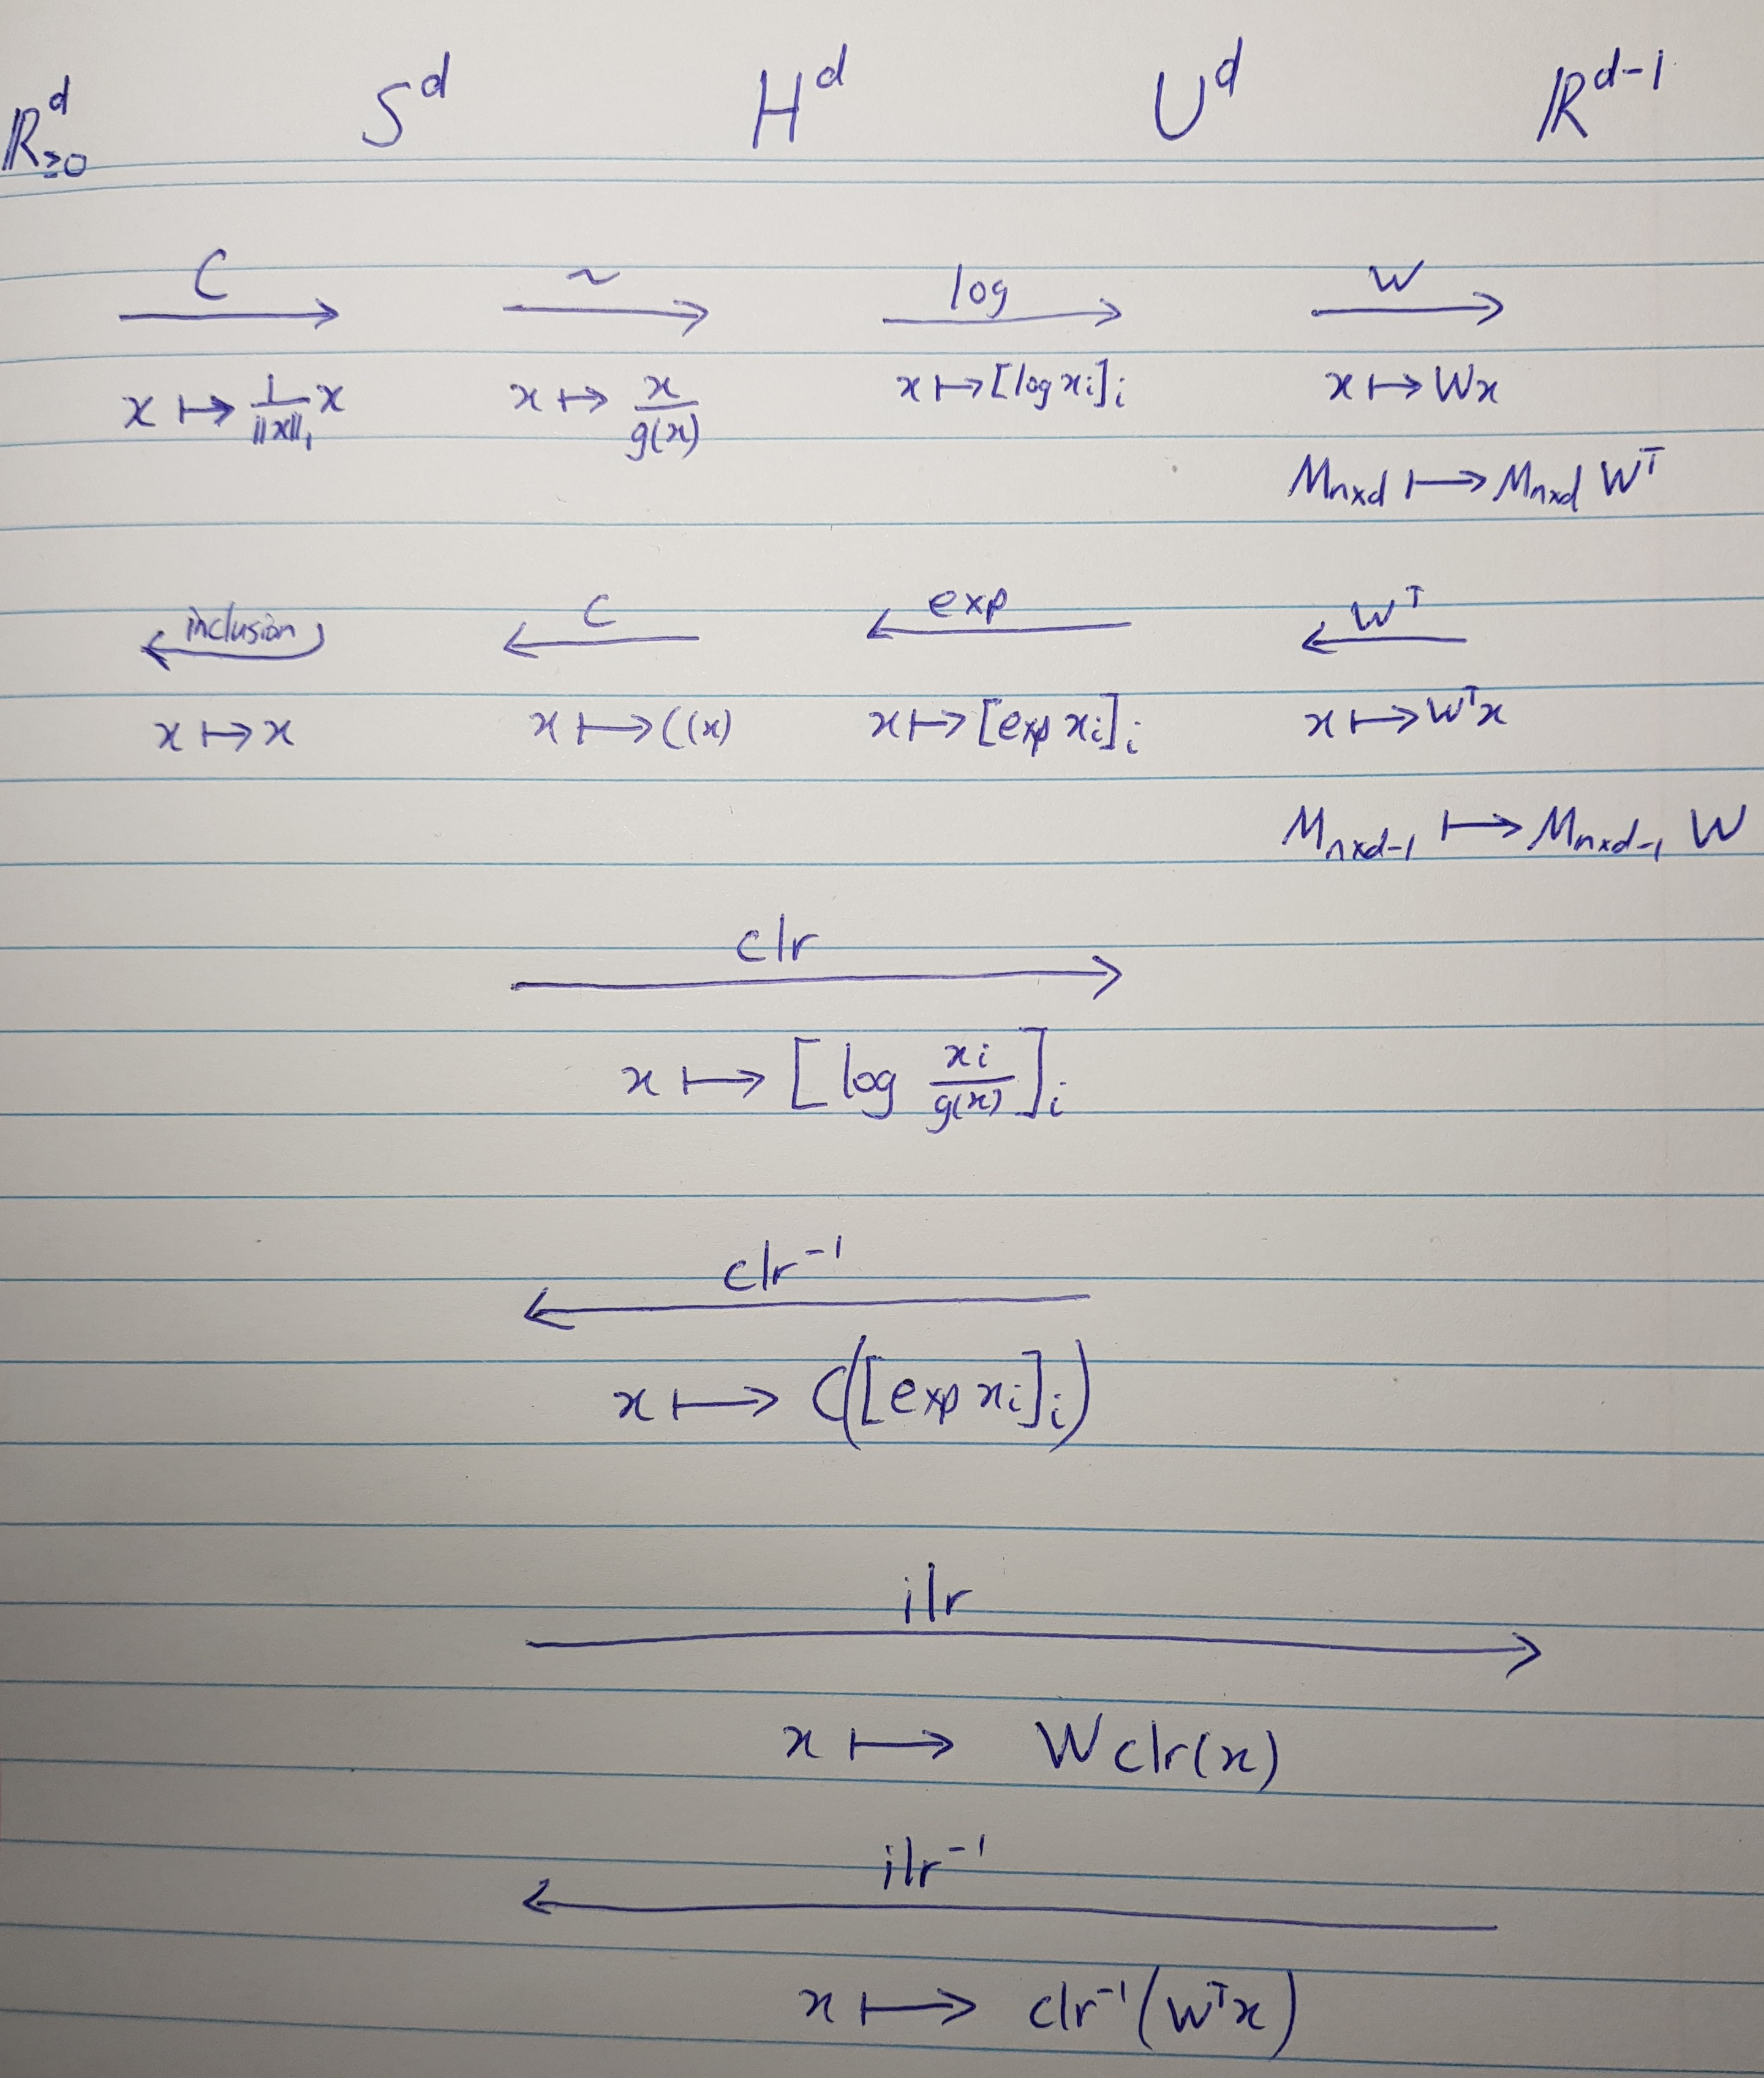
\includegraphics[scale=0.17]{./maps.jpg}
 % results.jpg: 0x0 pixel, 0dpi, nanxnan cm, bb=
\end{center}

\section{Hilbert Space Structure of the Aitchison Simplex}
Explicit forms of addition, scalar multiplication, inner product, norm, distance. 

Points in $S^d$ are subject to an equality condition and $d$ inequality conditions. The clr map reduces this to a single equality condition, and the ilr map further reduces this to no conditions at all. Thus, one approach for machine learning on CoDA is to transport the data to $\mathbb{R}^{d-1}$ via the ilr map, use a standard model in that space, and then transform back to $S^d.$ Empircally, this approach to dealing with CoDA has proved to be quite effective and has been considered as state of the art since the ilr transform was first proposed in (1984?) until quite recently. It addresses the points in the previous section about dealing specifically with CoDA and providing a vector space structure, a metric, and a full rank data matrix so that standard methods can be applied, but we still need to investigate whether other ways to model CoDA exist and on what types of CoDA such models are most effective on. 

\chapter{Information Geometry of the Probability Simplex}
[Expand background on statistical manifolds, FIM, KL-divergence, distance on Riemannian manifolds as geodesic distance...]
Each point in the probability simplex $\Delta^d$ corresponds naturally to a discrete probability distribution over $d$ states, so $\Delta^d$ can be viewed as a $d-1$ dimensional statistical manifold. A natural Riemannian metric for statistical manifolds is the Fisher information metric. The Fisher-Rao distance between two points on a statistical manifold as the distance between those points on the Riemannian manifold with metric given by the FIM. \
\\
\begin{Proposition}
The Fisher-Rao distance between $x,y \in \Delta^d$ is given by $$d_{FR}(x,y) = \arccos \left( \sum_{i=1}^d \sqrt{x_i y_i} \right).$$
\end{Proposition}

\begin{proof}
\end{proof}

\begin{Proposition}
As $p \to q$ in $\Delta^d,$ we have $D_{KL}(p, q) \sim 2 d_{FR}^2 (p,q).$ Thus, the KL divergence provides a local approximation to the Fisher-Rao distance.
\end{Proposition}

\begin{proof}
\end{proof}

\begin{Remark}
As $p\to e_i$ and $q\to e_j,$ $i\neq j,$ the KL divergence $D_{KL}(p,q)$ tends to infinity. Under the same conditions, $2 d_{FR}^2(p,q)$ approaches a finite value.  
\end{Remark}

\begin{Remark}
Suppose we have two models which approximates a composition $y \in \Delta^d$ with the same parameterised function $f_{\beta}(x_1,\ldots, x_m)$ and seek to find the $\beta\in \mathbb{R}^m$ which minimizes a loss function of the form $\ell  = \sum_{j=1}^m d(y_j, f_{\beta}(x_{j1}, \ldots, x_{jm}),$ with the only difference between the two models being the distance measures $d_1$ and $d_2.$ \
\\

Intuitively, we could expose a difference between the two models by using a dataset such that the labels are near points $p$ in the simplex $\Delta^d$ for which the difference between $d_1(p,q)$ and $d_2(p,q)$ (where $q$ is a point near $p$) is large compared to other areas of the simplex. Specifically (See Section 3.3 in the next chapter) in the case where $d_1$ is the KL divergence and $d_2$ is the Aitchison distance (i.e. the distance on $\Delta^d$ induced by the Euclidean distance on clr coordinates) , are such points related to points for which the Fisher Information Metric under clr coordinates is most dissimilar to the identity matrix? (And what is the correct notion of dissimilar?)    \
\\
As an example, take $x\in \Delta^d,$ $x= (1/d, \ldots, 1/d).$ Then $clr(x) = (0,\ldots, 0)$ and the FIM under clr coordinates is given by $\frac{1}{d} I_d - \frac{1}{d^2} \mathbf{1}_{d\times d}.$ What does this indicate exactly?
\\
Another example - Let $x = (0.998, 0.001, 0.001) \in \Delta^3.$ Then the FIM under the coordinates $\tilde{x}$ is approximately 
$$ \begin{bmatrix}1.2 \cdot 10^{-6} & 10^{-1}\\10^{-1} & 10^{-4} \end{bmatrix} $$
How should this be interpreted?
\end{Remark}


\chapter{Regression models on CoDA}


\section{Simple linear regression with CoDA feature and real prediction}
In (Combettes, Muller, Regression models for compositional data, 2019) they consider the case of predicting a real value with the independent variable being a single composition. In cases where the predicted values are real numbers, we can map the predictions onto $S^2$ by the inverse-ilr map so that we may consider an alternate loss function as implied by the previous chapter, but this is a forced unnatural connection to the Aitchison simplex and we do not expect improved information geometry by doing this. 

\section{Multiple linear regression with real features and CoDA prediction}
To predict one composition $z$ from $m$ independent real variables $x_k$, we can formulate the model 

$$ z = b_0 \oplus (\oplus_{k} x_k \otimes b_k)$$ and solve for the compositions $b_k.$ This is referred to as "Model 2" in (H. Wang, 2013). Similarly to the previous section, we can consider a new loss function which may give better information geometry.

\section{Multiple linear regression for CoDA features and CoDA prediction}
In (H. Wang et al, Multiple linear regression modeling for compositional data, 2013) the following regression model (clr-LR) is considered. Suppose we have labels $V$ and features $U^{(k)}, k=1,\ldots, m$ in $S^d_n,$ assumed to be centralized. Their model is given by $$ \hat{V} = \oplus_{k=1}^m \beta_k \otimes U^{(k)} $$

Let $Y = ilr(V), \hat{Y} = ilr(\hat{V}), X^{(k)} = ilr( U^{(k)} ).$  Since $ilr$ is an isometric isomorphism, we have $$ \hat{Y} = \sum_{k=1}^m \beta_k X^{(k)}.$$

To find $\beta \in \mathbb{R}^m,$ the authors minimize the Frobenius norm $ \| Y - \hat{Y} \|_F.$ [Derive closed form solution]. Following (Section 4.2 of) (M Avalos-Fernandez et al,  Representation Learning of Compositional Data, 2018), we expect that the model may have better information geometry if we consider minimizing the following loss instead:

$$ l_{CoDA} := D_{exp} \left( \sum_k \beta_k clr(U^{(k)} ), clr(V) \right)$$
$$ = (\mathbf{1}_{n \times 1})^T \exp \left( (\sum_i \beta_i X^{(i)})W \right) \mathbf{1}_{d\times 1} - \operatorname{trace}(\tilde{V}^T (\sum_i \beta_i X^{(i)})W )$$

Experimentally, evaluated on metrics on $\Delta^d$ such as Fisher-Rao distance, symmetric KL distance, L1 distance and L2 distance, these two models appear to be very similar, with CoDA-LR usually having 1 to 2 percent higher error than clr-LR. A goal is to design a dataset that causes these two models to show a greater disparity from one another and to understand why the might be so similar. 


\chapter*{Appendix}
.

%% Bibliography %%
\begin{thebibliography}{10}

    \bibitem{logodds}
   {\sc  A.~Banerjee}
    \newblock 'An Analysis of Logistic Models:
Exponential Family Connections and Online Performance'.
    \newblock {\em 2007 SIAM International Conference on Data Mining}
    2007.  
    

    

    \bibitem{mean}
    {\sc A.~Banerjee, X.~Gou, H.~Wang}
    \newblock  'On the Optimality of Conditional Expectation as a Bregman Predictor'
    \newblock {\em IEEE Trans. on Information Theory} Vol 51(7)
    2005.  
    
    \bibitem{Bi}
{\sc J.~ Borwein and A.~ Lewis}, {\em Convex Analysis and Nonlinear Optimization}, (2 ed.). Springer. p. 76, 2006.

\bibitem{Collins}
   {\sc  M.~Collins, R.E.~Schapire, Y.~Singer}
    \newblock 'Logistic Regression, AdaBoost and Bregman Distances'
    \newblock {\em Machine Learning}, 48(1/2/3).
    2002.
    

    \bibitem{pietra}
    {\sc S.~Della Pietra, V.~Della Pietra, J.~Lafferty}, 'Duality and Auxiliary Functions for Bregman Distances', {\em Tech. rep. CMU-CS-01-109, School of Computer Science, Carnegie Mellon University.} 2001.
    
\bibitem{GLM}
{\sc A.~J.~ Dobson and A.~G.~ Barnett}, {\em Introduction to Generalized Linear Models},  Boca Raton, FL: Chapman and Hall/CRC, 2008.


    \bibitem{Someone2000}
   {\sc  T.~Huang, M.~Gupta}
    \newblock Bregman distance to L1 regularized logistic regression.
    \newblock {\em International Conference on Pattern Recognition}
    2008.  
    

\bibitem{NEF}
{\sc C.~ Morris}, "Natural Exponential Families with Quadratic Variance Functions", Annals of Statistics,
10 (1), p65-80. 1982

\bibitem{flash}
{\sc F.~ Nielsen, V.~ Garcia}, "Statistical exponential families: A digest with flash cards", arXiv:0911.4863v2, 2011.

\bibitem{Cheng}
{\sc R.~ Nock, A.~ Menon and C.~ Ong}, "A scaled Bregman theorem with applications", NIPS'16 Proceedings of the 30th International Conference on Neural Information Processing Systems, p. 19-27, 2016. 




\end{thebibliography}


\end{document}

